%!TEX root = thesis.tex

\documentclass[12pt]{article}
\usepackage[spanish]{babel}

% Margenes
\usepackage{geometry}
\geometry{
  letterpaper,
  top=4cm,
  bottom=3cm,
  left=4cm,
  right=3cm
}

% Fuente
\usepackage{fontspec}
\setmainfont{Times New Roman}
\usepackage{csquotes}

\renewcommand{\baselinestretch}{1.5}

\usepackage{graphicx}
\usepackage{amsmath}
\usepackage{hyperref}
\usepackage{float}
\usepackage{parskip}
\usepackage[spanish]{cleveref}

\usepackage[caption = true]{subfig}

\usepackage[backend=biber,style=apa,language=spanish]{biblatex}
\bibliography{biblio}

\begin{document}

\title{Análisis Descriptivo y Predictivo Basado en Datos del Tráfico Vehicular en Antofagasta: Un Enfoque a partir de Reportes de Conductores}
\author{Richard Peña Bonifaz}
\date{\today}
\maketitle

\section*{Dedicatoria}

A todas las personas que estuvieron conmigo y me alentaron en los momentos más difíciles.

\section*{Reconocimientos}

A los profesores apasionados por su trabajo, que no solo transmiten conocimiento, sino también la pasión por el saber y la aplicación de la materia que imparten.

\newpage
\tableofcontents
\newpage

\section*{Resumen}

El presente proyecto tiene como propósito desarrollar una herramienta efectiva para analizar y predecir, con alta confiabilidad, el comportamiento del tráfico vehicular en la ciudad de Antofagasta mediante el uso de datos provenientes de la plataforma Waze Cities. Waze, a través de su comunidad de usuarios, ofrece información en tiempo real que permite obtener una visión detallada de los eventos de tráfico que ocurren en la ciudad. Esta investigación genera información relevante para la gestión del tráfico, facilitando la toma de decisiones por parte de las autoridades locales con el fin de mejorar la seguridad vial y optimizar la eficiencia del flujo vehicular. A través del análisis y explotación de estos datos, se identifican patrones y tendencias que, integrados en la planificación urbana, contribuirán a optimizar rutas críticas, reducir la congestión y minimizar la probabilidad de accidentes.

En este estudio se emplearán técnicas de análisis de datos y métodos geoespaciales mediante el uso de la librería GeoPandas en Python, además de la aplicación de series temporales para proporcionar visualizaciones claras y comprensibles dirigidas al usuario final. Adicionalmente, se implementarán técnicas de aprendizaje automático para realizar predicciones de tráfico, anticipándose a eventos y contribuyendo al desarrollo urbano eficiente y seguro \parencite{barcelo2005}.

\section{Introducción}
\subsection{Descripción del problema}

Antofagasta, una ciudad con más de 106,000 vehículos en circulación \parencite{comision2023}, enfrenta desafíos significativos en la gestión de su tráfico vehicular. Durante el año 2023, se registraron 1,715 accidentes, los cuales resultaron en 31 fallecidos y 102 heridos graves \parencite{comision2023}. La infraestructura vial limitada, sumada a la alta concentración de vehículos en un número reducido de arterias principales, agravó la congestión y elevó el riesgo de accidentes. A pesar de la existencia de estos problemas, no se cuenta con sistemas de monitoreo en tiempo real que permitan gestionar el tráfico de manera proactiva. Por ello, se aprovecharán fuentes de datos alternativas, como Waze, para recolectar información valiosa que facilite la toma de decisiones en materia de tráfico \parencite{chen2015}.

\subsection{Objetivo general}

Realizar un análisis exhaustivo del comportamiento del tráfico en la ciudad de Antofagasta basado en los eventos reportados por los conductores en la plataforma Waze. El objetivo final es generar información relevante que contribuya a la gestión eficiente del tráfico, mejorando la seguridad vial y optimizando el flujo vehicular.

\subsection{Objetivos específicos}

\begin{itemize}
    \item Obtener datos suficientes y representativos sobre los eventos de tráfico en Antofagasta mediante la API de Waze Cities.
    \item Realizar un análisis descriptivo de los datos recolectados para identificar patrones y tendencias relevantes en el comportamiento del tráfico.
    \item Identificar los factores clave que influyen en la seguridad vial y la eficiencia del tráfico en la ciudad.
    \item Presentar información visualmente comprensible y útil para las autoridades de gestión vial, facilitando la implementación de políticas y acciones basadas en datos \parencite{auld2009}.
    \item Utilizar los datos disponibles para desarrollar modelos predictivos de tráfico que permitan anticipar eventos y tomar decisiones proactivas en la gestión vial.
\end{itemize}

\section{Marco teórico}

El tráfico vehicular en entornos urbanos presenta un comportamiento complejo e impredecible, lo que dificulta su gestión eficiente. No obstante, el avance de las tecnologías móviles y la popularidad de aplicaciones como Waze permiten disponer de datos en tiempo real generados por los propios usuarios. Este proyecto se apoya en técnicas de análisis de datos y aprendizaje de máquinas (Machine Learning) para convertir esta información en herramientas útiles para la gestión vial. La utilización de datos geoespaciales, junto con la automatización de los procesos de recolección, análisis y visualización, constituye una solución costo-efectiva para mejorar la planificación del tráfico \parencite{barcelo2005}.

\subsection{Metodología}

Una de las principales limitaciones en el análisis de fenómenos es la ausencia de datos suficientes y debidamente estructurados. Por ello, se diseñó una estrategia de recolección de datos que garantizara conclusiones con un nivel adecuado de certeza. La API de Waze Cities, que proporciona información en tiempo real sobre eventos activos, fue la fuente principal de datos. Para lograr un volumen de datos representativo, se implementó un servidor encargado de recopilar y almacenar esta información de manera continua.

Se realizó un análisis geoespacial con el objetivo de identificar puntos críticos, como vías principales, calles secundarias y zonas de alto tráfico. Este análisis se llevó a cabo utilizando GeoPandas, una herramienta de Python especializada en operaciones geoespaciales. Además, se analizaron series temporales para detectar patrones y tendencias del tráfico, identificando estacionalidades en el comportamiento. Los resultados se presentaron mediante técnicas de visualización que permitieron interpretar las tendencias y puntos de interés de manera efectiva.

El pipeline de datos incluyó una base de datos relacional para almacenar los datos, un flujo ETL (Extract, Transform, Load) para procesarlos y un servidor web para visualizarlos. Se utilizó PostgreSQL como base de datos, APScheduler para la programación de tareas y Dash como herramienta de visualización. Este enfoque permitió automatizar el flujo de datos y garantizar la actualización constante de la información.

Adicionalmente, se entrenó un modelo de clasificación para determinar la probabilidad de ocurrencia de accidentes en diferentes puntos de la ciudad. El modelo seleccionado fue XGBoost, el cual fue seleccionado utilizando técnicas de validación cruzada y optimización de hiperparámetros. Los resultados obtenidos permitieron identificar las variables más influyentes en la ocurrencia de accidentes, así como la probabilidad de ocurrencia en diferentes condiciones de tráfico. Para la selección de variables se utilizó GridSearchCV, una técnica de búsqueda de hiperparámetros que permite encontrar la mejor combinación de variables para el modelo, se compararon modelos de regresión logística, árboles de decisión y XGBoost, siendo este último el que presentó el mejor desempeño en términos de precisión y sensibilidad.

Para la gestión del modelo, en cuanto a su implementación, mantenimiento y actualización, se programó con APSCheduler, una librería de tareas asíncronas en Python, que permite gestionar el ciclo de vida de los modelos de aprendizaje automático, desde su entrenamiento hasta su despliegue en producción y versionado.

En la parte del servidor, se desarrolló en Rust, un lenguaje de programación enfocado en la eficiencia en el uso de memoria y seguridad en el uso de la misma. Se utilizó la herramienta Memcached para generar un caché de los datos y de esta forma poder servirlos de manera más eficiente y rápida, debido al volumen de dato, se priorizó la unicidad de los datos, evitando generar copias, para no aumentar el uso de memoria.

Para el procesado de los datos en el cliente (Dash), se generan multiples workers que permiten servir la aplicación de forma eficiente, y se utiliza solo una instancia en memoria de los datos, compartidos por todos los datos, y para mantener la integridad de los datos, se implementó un Mutex para controlar el acceso de lectura a los mismos desde las tareas asíncronas.

La perspectiva general del flujo de datos se muestra en la \autoref{fig:fuente} y el flujo desde la API de Waze hasta el dashboard se puede observar en la \autoref{fig:wf_dash}

\begin{figure}[h]
    \centering
    \includegraphics[width=0.8\textwidth]{images/fuente_datos.png}
    \caption{Pipeline general de datos}
    \label{fig:fuente}
\end{figure}

\begin{figure}[h]
    \centering
    \includegraphics[width=0.8\textwidth]{images/wf_dash.png}
    \caption{Flujo de información en dashboard}
    \label{fig:wf_dash}
\end{figure}

\section{Desarrollo}

Para obtener los datos necesarios para el análisis, fue necesario generar un mecanismo para recolectar y almacenar la información de Waze Cities. Se implementó un servidor que se encarga de realizar peticiones a la API de Waze, recolectar los eventos de tráfico y almacenarlos en una base de datos PostgreSQL. Este servidor se ejecutaba de manera continua, actualizando la información cada 2 minutos. La estructura de la base de datos se muestra en la \autoref{fig:db_diagram}.

\begin{figure}[H]
    \centering
    \includegraphics[width=0.8\textwidth]{images/db_diagram.png}
    \caption{Diagrama de la base de datos}
    \label{fig:db_diagram}
\end{figure}

Existen dos estructuras principales, las alertas (alerts) y las congestiones (jams), el primero registra todos los eventos reportados por usuarios, tales como peligros, accidentes, congestión o rutas cerradas. En el caso de los eventos de congestión, son datos generados automáticamente por Waze, los cuales usando la geolocalización, estiman congestiones en diferentes puntos de la ciudad. Para este proyecto, se utilizó la información de las alertas. Sin embargo, se almacenaron los datos de congestión, para un posterior análisis, que está fuera del alcance de este estudio. Esta estructura se definió con base en los datos relevantes y completos que proporciona la API, los tipos de datos disponibles pueden ser consultados en la documentación de Waze \parencite{waze2024}.

Desde octubre de 2024 hasta abril de 2025, se han acumulado 40429 alertas, las cuales se analizarán a lo largo de este estudio.


\subsection{Eventos en el espacio y tiempo}

En la \autoref{fig:dist_events} se observa la distribución espacial de los distintos tipos de eventos en la ciudad. Se aprecia una mayor concentración en las principales avenidas, especialmente en el caso de los accidentes, los cuales tienden a ocurrir con mayor frecuencia en los cruces de estas arterias.

\begin{figure}[H]
    \centering
    \subfloat[Accidentes]{
        \includegraphics[width=0.33\textwidth]{images/dist_accidents.png}
    }
    \subfloat[Congestión]{
        \includegraphics[width=0.33\textwidth]{images/dist_jams.png}
    }
    \subfloat[Peligros]{
        \includegraphics[width=0.33\textwidth]{images/dist_hazards.png}
    }
    \caption{Distribución espacial de eventos en Antofagasta}
    \label{fig:dist_events}
\end{figure}

Para el análisis temporal, los eventos se agruparon por hora del día, calculando el promedio de eventos ocurridos por jornada. En la \autoref{fig:time_events} se evidencia una concentración de accidentes y congestiones durante las horas punta. En contraste, los eventos de tipo peligro presentan una distribución más uniforme a lo largo del día.

\begin{figure}[H]
    \centering
    \subfloat[Accidentes]{
        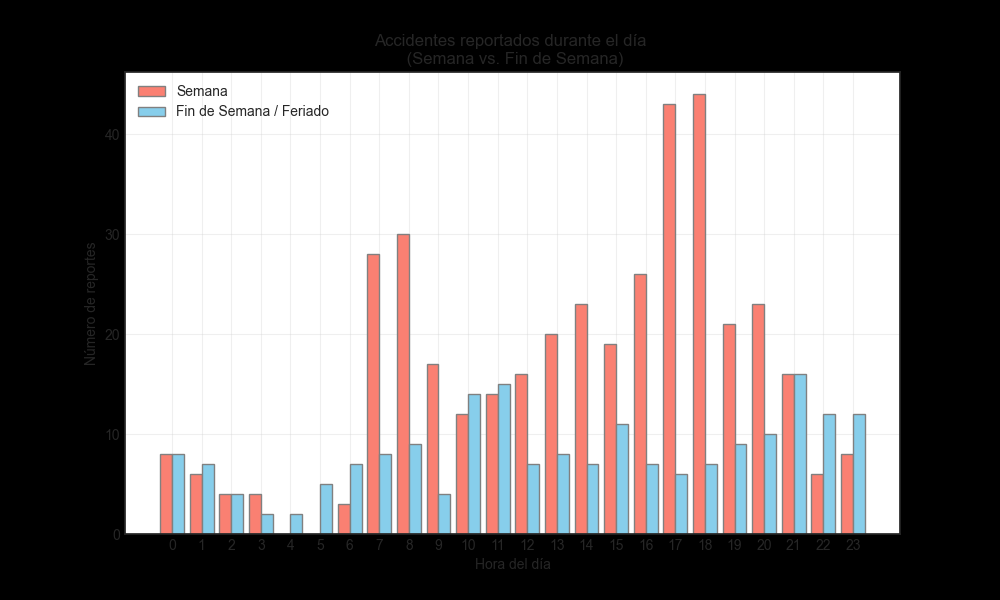
\includegraphics[width=0.6\textwidth]{images/ACCIDENT_per_hour.png}
    }
    \newline
    \subfloat[Congestión]{
        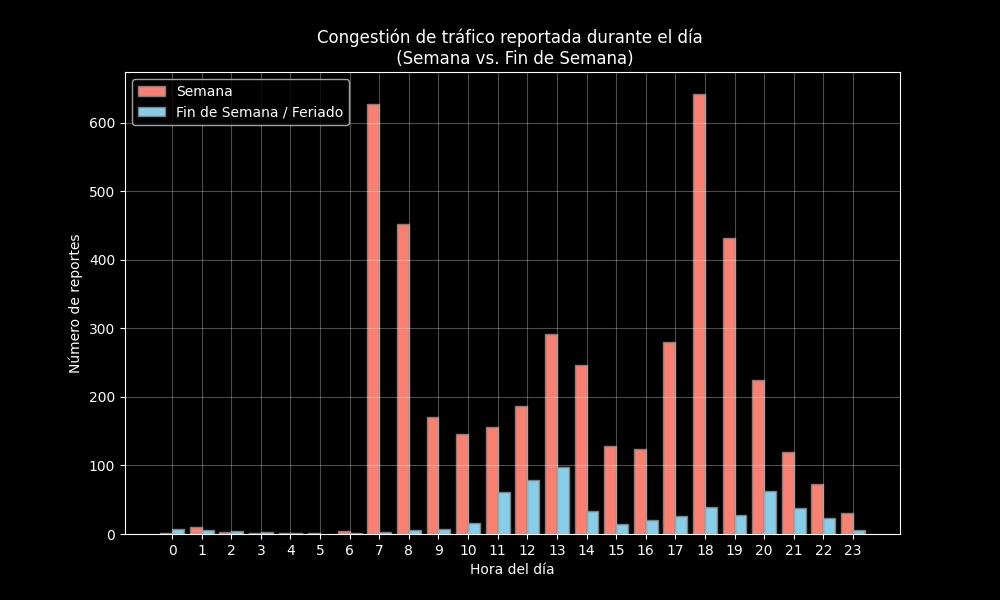
\includegraphics[width=0.6\textwidth]{images/JAM_per_hour.png}
    }
    \newline
    \subfloat[Peligros]{
        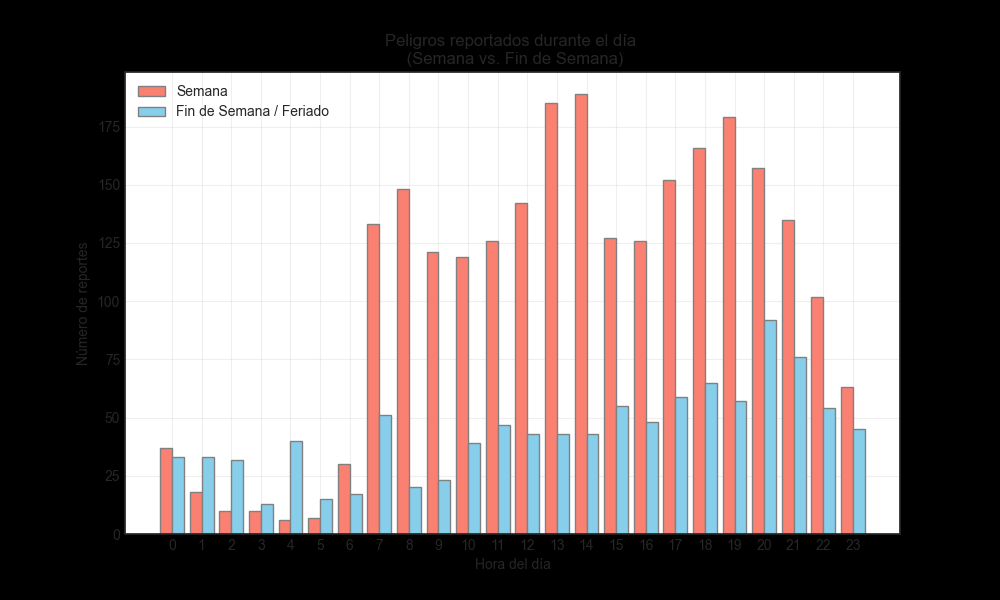
\includegraphics[width=0.6\textwidth]{images/HAZARD_per_hour.png}
    }
    \newline
    \caption{Eventos según hora del día en Antofagasta}
    \label{fig:time_events}
\end{figure}

\subsection{Modelo de correlación lineal}

Los resultados de la regresión lineal entre accidentes y reportes de congestión, presentados en la \autoref{fig:corr_lineal}, indican una fuerte correlación positiva durante los días de semana ($R^2 = 0.92$), lo que sugiere que a mayor número de reportes de congestión, también aumenta el número de accidentes. En cambio, durante los fines de semana la relación es más débil ($R^2 = 0.56$), aunque aún presente.

Estos resultados permiten postular una relación directa entre el flujo vehicular y la ocurrencia de accidentes, especialmente bajo condiciones de alta actividad urbana.

% Prueba hipótesis relación accidents-jams

\begin{figure}[H]
    \centering
    \subfloat[Día de semana]{
        \includegraphics[width=0.9\textwidth]{images/corr_lin_ds.png}
    }
    \newline
    \subfloat[Fin de semana]{
        \includegraphics[width=0.9\textwidth]{images/corr_lin_fs.png}
    }
    \newline
    \caption{Correlación lineal entre accidentes y congestión}
    \label{fig:corr_lineal}
\end{figure}

\subsection{Prueba de hipótesis de correlación lineal}

Para evaluar la existencia de una relación estadísticamente significativa entre el número de reportes de congestión y la cantidad de accidentes por hora, se aplicó una prueba de correlación de Pearson.

La hipótesis nula ($H_0$) establece que no existe correlación lineal entre ambas variables, mientras que la hipótesis alternativa ($H_1$) plantea que sí existe tal correlación:

\begin{align}
H_0&:\ \rho = 0 \\
H_1&:\ \rho \ne 0
\end{align}

Donde $\rho$ representa el coeficiente de correlación poblacional. El estadístico de prueba se calcula mediante:

\begin{equation}
t = \frac{r \sqrt{n - 2}}{\sqrt{1 - r^2}}
\end{equation}

donde $r$ es el coeficiente de correlación muestral y $n$ el número de observaciones. El valor resultante se contrasta con la distribución t de Student con $n - 2$ grados de libertad.

El análisis estadístico del modelo lineal entregó resultados significativos tanto para días de semana como para fin de semana:

\begin{itemize}
    \item Para días de semana:
    \begin{itemize}
        \item El modelo ajustado fue $y = 0.1054x + 0.1824$
        \item Se obtuvo un $R^2 = 0.92$, explicando el 92\% de la variabilidad
        \item El coeficiente de correlación de Pearson fue $r = 0.96$ con IC 95\%: [0.91, 0.98]
        \item La significancia global fue $F(1, 22) = 256.29$, $p < 0.0001$
        \item Los parámetros fueron estadísticamente significativos con $p < 0.001$
        \item El estadístico $t$ para la prueba de correlación fue $t = 16.01$, $p < 0.0001$
    \end{itemize}

    \item Para fines de semana:
    \begin{itemize}
        \item El modelo ajustado fue $y = 0.1042x + 0.1078$
        \item Se obtuvo un $R^2 = 0.56$, explicando el 56\% de la variabilidad
        \item El coeficiente de correlación de Pearson fue $r = 0.75$ con IC 95\%: [0.49, 0.88]
        \item La significancia global fue $F(1, 22) = 27.74$, $p < 0.0001$
        \item Los parámetros fueron estadísticamente significativos con $p < 0.0001$
        \item El estadístico $t$ para la prueba de correlación fue $t = 5.27$, $p < 0.0001$
    \end{itemize}
\end{itemize}

Estos resultados permiten rechazar la hipótesis nula con un nivel de confianza del 99\%, confirmando la existencia de una relación lineal estadísticamente significativa entre el número de reportes de congestión y la cantidad de accidentes registrados por hora.

\begin{figure}[H]
\centering
\includegraphics[width=0.9\textwidth]{images/residuos_lin.png}
\caption{Residuos del modelo lineal para días de semana y fines de semana}
\label{fig:resid_lin}
\end{figure}

\begin{figure}[H]
\centering
\includegraphics[width=0.9\textwidth]{images/qq_lin.png}
\caption{Gráficos Q-Q de los residuos del modelo lineal}
\label{fig:qq_lin}
\end{figure}

Los gráficos Q-Q (\autoref{fig:qq_lin}) muestran una aproximación razonable a la distribución normal en ambos períodos. Para los días de semana, los puntos siguen la línea de referencia bastante bien, con pequeñas desviaciones en los extremos. En el caso de fin de semana, aunque también hay una tendencia lineal, se observan algunas desviaciones más notables en los valores centrales.

Los gráficos de residuos (\autoref{fig:resid_lin}) revelan patrones distintos para cada período. En días de semana, aunque hay cierta dispersión alrededor de cero, se observa variabilidad considerable con algunos residuos positivos destacados (especialmente entre valores ajustados de 0.5 y 1.25) y residuos negativos pronunciados en valores extremos. Para fines de semana, los residuos muestran menor magnitud global pero un patrón menos aleatorio, sugiriendo posible estructura no capturada por el modelo lineal.

En resumen, el análisis confirma una relación lineal significativa entre congestión y accidentes, considerablemente más fuerte durante días laborables ($R^2 = 0.92$) que en fines de semana ($R^2 = 0.56$). Los patrones observados en los residuos, particularmente para fines de semana, sugieren la pertinencia de explorar modelos no lineales que podrían capturar mejor las relaciones subyacentes en los datos.


\subsection{Modelo de correlación exponencial inversa}

Dado que la relación entre congestión y accidentes no necesariamente es lineal en todos los contextos —especialmente bajo alta densidad vehicular— se propuso un modelo de potencia inversa. Este considera que, a medida que aumenta la congestión (y por ende, disminuye la velocidad promedio), podría reducirse la probabilidad de accidentes graves.

El modelo propuesto se ajusta a la siguiente forma funcional:

\begin{equation}
A(x) = \frac{\alpha}{x^{\beta}} + \gamma
\end{equation}

donde:
\begin{itemize}
    \item $A(x)$ es el número estimado de accidentes por hora,
    \item $x$ representa el número de reportes de congestión por hora,
    \item $\alpha$, $\beta$ y $\gamma$ son parámetros ajustados mediante regresión no lineal.
\end{itemize}

Este modelo fue aplicado tanto a los días de semana como a los fines de semana. En ambos casos, se observó un buen ajuste visual, respaldando la hipótesis de una relación decreciente no lineal entre ambas variables bajo ciertas condiciones de tráfico.

Los resultados del ajuste se presentan en la \autoref{fig:corr_exp}, mostrando un ajuste significativo del modelo a los datos.

\begin{figure}[H]
    \centering
    \subfloat[Día de semana]{
        \includegraphics[width=0.9\textwidth]{images/corr_exp_ds.png}
    }
    \newline
    \subfloat[Fin de semana]{
        \includegraphics[width=0.9\textwidth]{images/corr_exp_fs.png}
    }
    \newline
    \caption{Correlación de potencia inversa entre accidentes y congestión}
    \label{fig:corr_exp}
\end{figure}

El análisis estadístico del modelo de potencia inversa entregó resultados significativos tanto para días de semana como para fin de semana:

\begin{itemize}
    \item Para días de semana:
    \begin{itemize}
        \item El modelo ajustado fue $y = 0.2962/x^{0.6415}$
        \item Se obtuvo un $R^2 = 0.96$, explicando el 96\% de la variabilidad
        \item La significancia global fue $F(2, 22) = 263.68$, $p < 0.0001$
        \item Los parámetros fueron estadísticamente significativos con $p < 0.0001$
    \end{itemize}

    \item Para fines de semana:
    \begin{itemize}
        \item El modelo ajustado fue $y = 0.2206/x^{0.2512}$
        \item Se obtuvo un $R^2 = 0.55$, explicando el 55\% de la variabilidad
        \item La significancia global fue $F(2, 22) = 13.41$, $p < 0.001$
        \item Los parámetros fueron estadísticamente significativos con $p < 0.001$
    \end{itemize}
\end{itemize}

Este análisis revela diferencias importantes en la dinámica de la relación congestión-accidentes entre períodos. Durante los días de semana, el exponente negativo de mayor magnitud ($-0.6415$) indica una relación más sensible entre las variables, mientras que en fines de semana el exponente menor ($-0.2512$) sugiere una relación menos pronunciada.

\begin{figure}[H]
\centering
\includegraphics[width=0.9\textwidth]{images/residuos_exp.png}
\caption{Residuos del modelo de potencia inversa para días de semana y fines de semana}
\label{fig:resid_exp}
\end{figure}

\begin{figure}[H]
\centering
\includegraphics[width=0.9\textwidth]{images/qq_exp.png}
\caption{Gráficos Q-Q de los residuos del modelo de potencia inversa}
\label{fig:qq_exp}
\end{figure}

Los gráficos de residuos (\autoref{fig:resid_exp}) muestran una dispersión aleatoria en torno a cero, sin evidencias claras de heterocedasticidad ni patrones sistemáticos, lo que respalda la validez del ajuste no lineal propuesto. En particular, para los días de semana, los residuos muestran una mayor variabilidad con valores extremos más pronunciados (entre -0.15 y 0.3), en comparación con los fines de semana, donde la dispersión es menor (aproximadamente entre -0.1 y 0.15).

Complementariamente, los gráficos Q-Q (\autoref{fig:qq_exp}) revelan una aproximación a la distribución normal de los residuos en ambos casos, aunque con algunas desviaciones. En días de semana, se observan desviaciones notables en ambos extremos, particularmente en los valores positivos más altos, sugiriendo colas más pesadas que la distribución normal. Para los fines de semana, la alineación con la línea teórica es mejor en los valores centrales, con desviaciones más leves en los extremos.

En conjunto, estos resultados indican que el modelo de potencia inversa no solo es estadísticamente significativo, sino que además presenta supuestos de ajuste razonablemente válidos en términos de normalidad de residuos, lo que fortalece la hipótesis de una relación decreciente entre la congestión y la probabilidad de accidentes graves en contextos urbanos.

% Cálculo de la frecuencia por zona
% Filtro por zona
%    Algóritmo cKDTree

\subsection{Frecuencia por zona}

Para representar conjuntos estáticos de puntos espaciales, se utiliza la estructura cKd-tree, una variante compacta del Kd-tree que codifica distancias relativas mediante spiral codes y las almacena usando Directly Addressable Codes (DACs), optimizando el uso de memoria sin sacrificar eficiencia en consultas espaciales \parencite{gutierrez2023ckdtree}. A cada zona la llamaremos cuadrante o segmento.

En la \autoref{fig:quad_acc} se puede ver cómo se distribuyen los segmentos numéricamente, comenzando desde el segmento 1 en la esquina inferior izquierda. La opacidad del color rojo está relacionada con la cantidad de accidentes por segmento.

\begin{figure}[H]
    \centering
    \includegraphics[width=0.38\textwidth]{images/quad_acc.png}
    \caption{Identificación de cuadrantes en mapa de Antofagasta}
    \label{fig:quad_acc}
\end{figure}

Tomamos la media de accidentes diarios, los agrupamos por segmento, definimos que las zonas mayores a 0.8 accidentes por día son considerados críticos, construimos un mapa según la criticidad (\autoref{fig:quad_mean_day}), si tomamos la suma de los accidentes, tenemos la \autoref{fig:quad_acc_total} que muestra la cantidad de accidentes reportados en el segmento en el periodo de estudio, que a su vez se clasifican como críticos si poseen más de 140 accidentes.


\begin{figure}[H]
    \centering
    \subfloat[Media de accidentes por día]{
        \includegraphics[width=0.5\textwidth]{images/quad_mean_day_color.png}
        \label{fig:quad_mean_day}
    }
    \subfloat[Total accidentes]{
        \includegraphics[width=0.5\textwidth]{images/quad_acc_color.png}
        \label{fig:quad_acc_total}
    }
    \caption{Accidentes por segmento}
\end{figure}


% Ruta más segura

% Machine learning (XGBoost)

\subsection{Selección del modelo de Machine Learning}

Se evaluaron distintos algoritmos de clasificación para abordar el problema planteado. Inicialmente, se probaron modelos clásicos como \textit{Logistic Regression}, \textit{K-Nearest Neighbors}, \textit{Decision Tree}, entre otros. Sin embargo, estos no mostraron mejoras relevantes en las métricas evaluadas, por lo que se descartaron para la fase de ajuste de hiperparámetros.

Se procedió entonces a aplicar una búsqueda exhaustiva (\textit{GridSearchCV}) sobre dos modelos con buen desempeño preliminar: \textbf{Random Forest} y \textbf{XGBoost}.

\paragraph{Random Forest.}
Se evaluaron los siguientes hiperparámetros:

\begin{itemize}
    \item \texttt{max\_depth}: [2, 5, 10]
    \item \texttt{n\_estimators}: [20, 80, 100, 200]
    \item \texttt{min\_samples\_leaf}: [2, 4, 8]
    \item \texttt{max\_leaf\_nodes}: [2, 8]
    \item \texttt{max\_features}: [2, 8]
    \item \texttt{class\_weight}: [None, 'balanced']
\end{itemize}

Los mejores hiperparámetros obtenidos fueron:

\begin{itemize}
    \item \texttt{class\_weight}: None
    \item \texttt{max\_depth}: 10
    \item \texttt{max\_features}: 2
    \item \texttt{max\_leaf\_nodes}: 8
    \item \texttt{min\_samples\_leaf}: 2
    \item \texttt{n\_estimators}: 100
\end{itemize}

Con estos valores, el modelo alcanzó una puntuación máxima de \textbf{0.7957} en validación cruzada.


\paragraph{XGBoost.}
Se aplicaron múltiples rondas de \textit{grid search} con distintos rangos de hiperparámetros, refinando progresivamente los valores. Los mejores resultados se obtuvieron con:

\begin{itemize}
    \item \texttt{colsample\_bytree}: 0.7
    \item \texttt{gamma}: 1
    \item \texttt{learning\_rate}: 0.1
    \item \texttt{max\_depth}: 30
    \item \texttt{n\_estimators}: 80
\end{itemize}

Este modelo logró una métrica de validación cruzada de \textbf{0.8665}, superando significativamente al resto de las alternativas evaluadas. Por este motivo, \textbf{XGBoost fue seleccionado como modelo final}.

En el \autoref{tab:model-comparison} se puede observar la comparación de ambos modelos.

\begin{table}[H]
\centering
\begin{tabular}{|l|p{9cm}|c|}
\hline
\textbf{Modelo} & \textbf{Mejores Hiperparámetros} & \textbf{Mejor Score} \\
\hline
\textbf{Random Forest} &
\begin{tabular}[c]{@{}l@{}}
\texttt{class\_weight}: None\\
\texttt{max\_depth}: 10\\
\texttt{max\_features}: 2\\
\texttt{max\_leaf\_nodes}: 8\\
\texttt{min\_samples\_leaf}: 2\\
\texttt{n\_estimators}: 100
\end{tabular}
& 0.7957 \\
\hline
\textbf{XGBoost} &
\begin{tabular}[c]{@{}l@{}}
\texttt{colsample\_bytree}: 0.7\\
\texttt{gamma}: 1\\
\texttt{learning\_rate}: 0.1\\
\texttt{max\_depth}: 30\\
\texttt{n\_estimators}: 80
\end{tabular}
& \textbf{0.8665} \\
\hline
\end{tabular}
\caption{Comparativa de modelos ajustados con GridSearchCV}
\label{tab:model-comparison}
\end{table}


\subsection{Generación de eventos negativos simulados} \label{ssec:class_balancing}

Dado que el conjunto original contenía únicamente eventos positivos (ocurridos), fue necesario generar instancias negativas (no ocurridos) para entrenar un modelo de clasificación binaria. Para ello, se implementó una estrategia inspirada en el enfoque de generación de eventos negativos artificiales propuesto por Goedertier et al. (2009), que permite representar problemas secuenciales como tareas de clasificación supervisada.

En nuestro caso, la generación se basa en una grilla temporal con intervalos de 5 minutos, sobre la cual se combinan todas las posibles ubicaciones (\texttt{group}) y tipos de evento. Luego, se identifican aquellas combinaciones que no se encuentran en los datos originales (es decir, donde no ocurrió un evento) y se etiquetan como eventos negativos (\texttt{happen} = 0). Estas instancias se muestrean de forma aleatoria para igualar la cantidad de eventos positivos, logrando así un conjunto balanceado con un 50\% de eventos positivos y 50\% de negativos.

Este enfoque permite mantener la estructura temporal y geoespacial de los datos reales, evitando introducir ruido aleatorio, y facilitando la evaluación robusta de métricas como \texttt{recall} y \texttt{precision} \parencite{goedertier2009robust}.


\subsection{Resultados del modelo seleccionado}

La versión final del modelo (\texttt{v6}) se entrenó utilizando los hiperparámetros obtenidos durante la etapa de validación cruzada. El modelo fue registrado y versionado mediante \textit{MLflow}, permitiendo un seguimiento detallado de sus parámetros y métricas.

\noindent Los parámetros más relevantes del modelo fueron:

\begin{itemize}
    \item \texttt{max\_depth} = 20
    \item \texttt{n\_estimators} = 80
    \item \texttt{learning\_rate} = 0.1
    \item \texttt{gamma} = 0.8
    \item \texttt{colsample\_bytree} = 0.7
\end{itemize}

El modelo utiliza codificación \textit{one-hot} y un esquema de clasificación binaria (\texttt{binary:logistic}), con una semilla aleatoria (\texttt{random\_state = 42}) para garantizar la reproducibilidad.


\noindent En cuanto al rendimiento, se obtuvieron los siguientes resultados para una muestra de 64.708 eventos, con un 50\% de eventos ocurridos y un 50\% de no ocurridos. Esta proporción se logró mediante la simulación de eventos negativos sobre una grilla temporal de 5 minutos, generando combinaciones posibles de tiempo, localización y tipo de evento que no están presentes en los datos originales (\autoref{ssec:class_balancing}). Esto permite evaluar el modelo en condiciones balanceadas, facilitando la interpretación de métricas como \texttt{precision}, \texttt{recall} y \texttt{F1-score}.

\begin{itemize}
    \item \textbf{Accuracy}: 0.8795
    \item \textbf{Recall}: 0.9076
    \item \textbf{Precision}: 0.8583
    \item \textbf{F1-score}: 0.8823
    \item \textbf{Promedio validación cruzada (10 folds)}: 0.7819
\end{itemize}

\noindent Respecto a la matriz de confusión, se registraron los siguientes valores:

\begin{itemize}
    \item Verdaderos positivos: 5,539
    \item Verdaderos negativos: 5,843
    \item Falsos positivos: 965
    \item Falsos negativos: 595
\end{itemize}

Estas métricas evidencian un modelo con excelente capacidad para identificar correctamente los casos positivos, sin sacrificar precisión ni equilibrio. La validación cruzada muestra estabilidad a lo largo de los distintos folds, lo que refuerza la robustez del modelo final y confirma que no hubo sobreentrenamiento.

\subsection{Curva de aprendizaje del modelo}

La \autoref{fig:learning_curve} muestra la curva de aprendizaje del modelo XGBoost entrenado. Se observa un rendimiento alto y consistente tanto en el conjunto de entrenamiento como en el de validación (aproximadamente 0.88–0.90), con una brecha mínima entre ambas curvas. Esto indica que el modelo generaliza adecuadamente, sin presentar sobreajuste ni subajuste. Además, el comportamiento plano de ambas curvas sugiere que incrementar el tamaño del conjunto de entrenamiento no tendría un impacto significativo en el rendimiento, lo cual evidencia una saturación en la capacidad de aprendizaje del modelo con las características actuales.


\begin{figure}[H]
    \centering
    \includegraphics[width=0.8\textwidth]{images/learning_curve.png}
    \caption{Identificación de cuadrantes en mapa de Antofagasta}
    \label{fig:learning_curve}
\end{figure}

% Aplicación implementacióñ (dashboard online y ML)

\subsection{Despliegue y mantenimiento del modelo}

Para entregar una interfaz que permita al usuario final interactuar con los datos, se desarrolló un tablero de control utilizando Dash \parencite{dashboard2024}, un marco de trabajo especializado en la presentación de datos gráficos mediante Python. La arquitectura del sistema se diseñó considerando dos componentes principales: un servidor implementado en Rust y un cliente en Python, como se muestra en la \autoref{fig:architecture}. El servidor se encarga de las operaciones intensivas como la captura, transformación, almacenamiento y gestión del caché de los datos, mientras que el cliente maneja la interacción con el usuario, la actualización de datos desde el servidor, el entrenamiento del modelo y la generación del tablero de control.

El ciclo de vida del modelo se gestiona mediante APScheduler, una biblioteca de Python especializada en la programación de tareas asíncronas. Esta herramienta permite automatizar el reentrenamiento periódico del modelo con nuevos datos, garantizando su actualización y adaptación a los cambios en los patrones de tráfico. El proceso incluye la validación automática del rendimiento del modelo, comparando las métricas clave (precisión, recall, F1-score) con los umbrales establecidos, y solo se despliega una nueva versión si representa una mejora significativa.

La implementación del servidor en Rust aprovecha las ventajas del lenguaje en cuanto a eficiencia y seguridad en el manejo de memoria. Se utiliza Memcached como sistema de caché para optimizar el acceso a los datos frecuentemente consultados, implementando una estrategia de almacenamiento que prioriza la unicidad de los datos para minimizar el uso de memoria. En el lado del cliente, se implementa un sistema de workers múltiples que comparten una única instancia de los datos en memoria, protegida mediante un mutex para garantizar la integridad en las operaciones de lectura concurrentes.

\begin{figure}[H]
    \centering
    \includegraphics[width=0.8\textwidth]{images/dashboard.png}
    \caption{Arquitectura del sistema}
    \label{fig:architecture}
\end{figure}

El entrenamiento del modelo está programado para realizarse cada 30 días, utilizando los nuevos datos. Los datos del dashboard se actualizan cada 5 minutos.


\section{Resultados}

Los análisis espaciales y temporales realizados permitieron identificar patrones críticos en la ocurrencia de accidentes en Antofagasta. En la \autoref{fig:quad_acc_total} se observan las zonas con mayor concentración de accidentes, destacando claramente los segmentos ubicados en el eje de la avenida Pedro Aguirre Cerda, especialmente en el cruce con Nicolás Tirado (segmentos 106 a 109). Este corredor vial presenta una densidad particularmente alta, lo que lo posiciona como un foco de atención prioritaria.

Asimismo, se identificó un segundo punto crítico en la intersección entre la Avenida Salvador Allende y Edmundo Pérez Zujovic, donde convergen flujos de alto volumen provenientes del norte y del centro de la ciudad. Esta área (segmentos 84 y 103) también mostró una alta frecuencia de accidentes diarios, como se observa en la \autoref{fig:quad_mean_day}.

El centro de la ciudad, particularmente en segmento 82, evidenció una densidad considerable de accidentes.

Los modelos estadísticos desarrollados mostraron una fuerte correlación entre congestión y accidentes, especialmente durante los días de semana. El modelo de potencia inversa entregó un mejor ajuste ($R^2 = 0.96$) que el modelo lineal ($R^2 = 0.92$), capturando de mejor forma la dinámica decreciente del riesgo bajo alta congestión.

Finalmente, el modelo predictivo XGBoost alcanzó un desempeño sobresaliente (\textbf{F1-score = 0.8823}, \textbf{Recall = 0.9076}), confirmando su utilidad como herramienta predictiva y de soporte en la toma de decisiones en gestión vial.

% Observaciones y resultados del estudio

% \section{Discusión}

% Preguntas y posibles soluciones

\section{Conclusiones}

Este estudio demuestra la factibilidad y el impacto del uso de datos colaborativos para la gestión inteligente del tráfico urbano. A través de una arquitectura eficiente y una metodología robusta, se logró:

\begin{itemize}
    \item Identificar zonas críticas con alta concentración de accidentes, como el cruce de Nicolás Tirado con Pedro Aguirre Cerda, la intersección de Salvador Allende con Edmundo Pérez Zujovic, y sectores del centro de Antofagasta.
    \item Confirmar la existencia de una relación estadísticamente significativa entre los reportes de congestión y los accidentes, siendo más fuerte durante los días de semana.
    \item Validar el uso de modelos no lineales como herramientas más adecuadas para representar fenómenos de tráfico en contextos urbanos densos.
    \item Desarrollar un modelo predictivo basado en XGBoost con alto rendimiento, capaz de anticipar la ocurrencia de accidentes con gran precisión.
    \item Implementar un sistema funcional de monitoreo y visualización que permite actualizar el modelo periódicamente y ofrecer datos en tiempo real a los usuarios finales.
\end{itemize}

Se concluye que el enfoque propuesto no solo es viable, sino escalable, y representa una base sólida para iniciativas de movilidad urbana basadas en datos.

\section{Recomendaciones}

A partir de los resultados obtenidos, se proponen las siguientes recomendaciones para autoridades locales, planificadores urbanos y futuras investigaciones:

\begin{itemize}
    \item \textbf{Intervención en zonas críticas}: Priorizar acciones de ingeniería vial, señalización y fiscalización en los segmentos identificados como críticos, particularmente en el eje Pedro Aguirre Cerda, Salvador Allende y el centro de la ciudad.
    \item \textbf{Monitoreo continuo}: Mantener y escalar el sistema de recolección y análisis de datos, integrando nuevas fuentes (sensores, cámaras) para enriquecer el modelo.
    \item \textbf{Validación en terreno}: Complementar los hallazgos con estudios de campo para confirmar condiciones geométricas, flujos vehiculares y comportamiento de los usuarios en las zonas críticas.
    \item \textbf{Extensión del sistema}: Replicar esta metodología en otras ciudades de tamaño medio que carezcan de infraestructura de monitoreo formal.
    \item \textbf{Nuevas líneas de investigación}: Incorporar variables climáticas, de infraestructura o comportamiento humano para enriquecer los modelos predictivos y explorar algoritmos más avanzados (LSTM, transformers, modelos causales).
\end{itemize}

Estas recomendaciones apuntan a fortalecer una gestión vial basada en datos, proactiva y centrada en la seguridad de los ciudadanos.

\newpage
\printbibliography

\end{document}

